\clearpage
\section{Using Input and Output} % (fold)
\label{sec:using_input_and_output}

Using File Input and Output it is now possible to load and save data. As an example we will examine how you can go about saving and loading data in the small db program.

\subsection{Saving Data from Small DB} % (fold)
\label{ssub:saving_data_from_small_db}

The Small DB\footnote{In this chapter we will be saving data from the array based version of the Small DB program, though a similar approach would be taken to save the linked version.} program allows the user to enter a number of \emph{row} values, with each row having a single column that stores a data value (either an integer, text, or double value). At this stage the program only keeps its data while it is executing, once it ends the data is gone. The first step is therefore to save the data from the program into a file.

\subsubsection{Row File Format} % (fold)
\label{ssub:row_file_format}

When thinking about saving data the first task is to try to determine how the data can be saved so that it can later be read back into the program. The following information can help us design the structure of the file saved from the program: 

\begin{enumerate}
  \item There are a variable number of rows.
  \item Each row has a fixed size, when you know the kind of data it is storing.
\end{enumerate}

In the array based version of the Small DB program the number of rows is stored in the \texttt{data store}. Saving this data to file can be achieved by saving the number of rows before storing the data from each row. This will mean that when the file is loaded the program can read the number of rows, and use this information to create enough space for these in memory before reading them from the file. \fref{fig:row-file-struct} shows an example of the file structure saved from the program.

\begin{figure}[h]
   \centering
   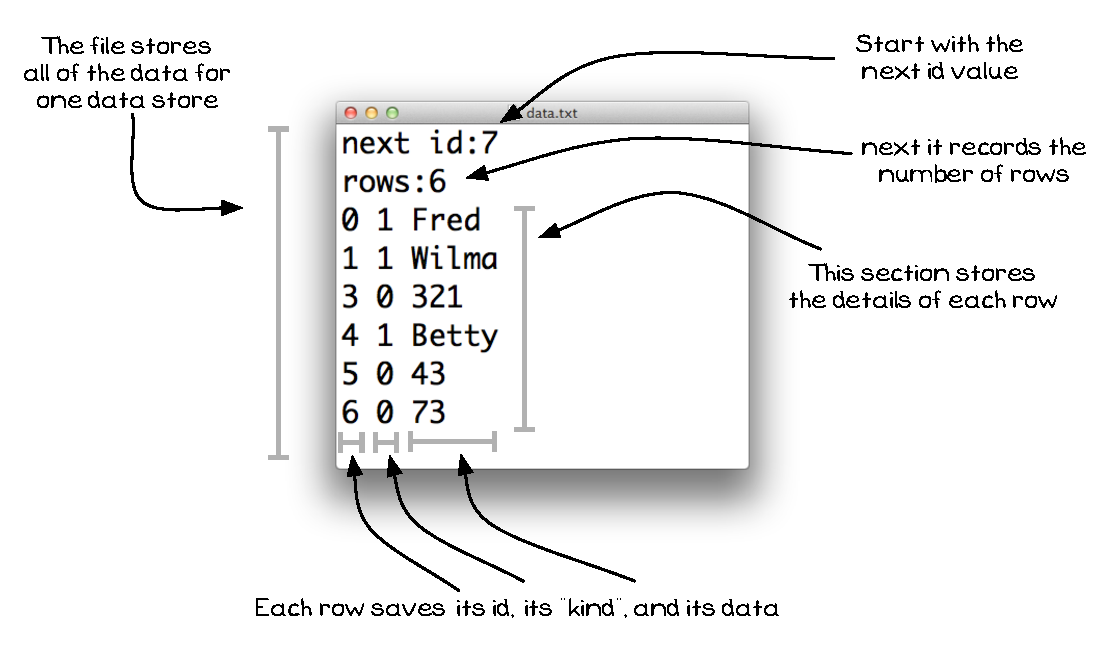
\includegraphics[width=\textwidth]{./topics/file-io/diagrams/RowFileStructure} 
   \caption{The structure of the Small DB data file}
   \label{fig:row-file-struct}
\end{figure}

% subsubsection row_file_format (end)

\subsubsection{Saving the Data Store} % (fold)
\label{ssub:saving_the_data_store}

The pseudocode in \lref{plst:save} shows the steps that can be followed to save the data from a data store into a file. Notice that the number of rows is being saved into the file, before the row data. This will make it easier to load the file back into memory.

\pseudocode{plst:save}{Pseudocode for Save (for Small DB array version)}{topics/file-io/application/save_data_store.txt}

The \texttt{Save} procedure calls a \texttt{Write Row to File} procedure to store each row in the file. The pseudocode for this procedure is shown in \lref{plst:save_row}. This code saves the \texttt{id} and \texttt{kind} values to the file, and then uses a \nameref{sub:case_statement} to ensure it saved the correct value from the \texttt{row}'s data.

\pseudocode{plst:save_row}{Pseudocode for the \texttt{Write Row to File} procedure (for Small DB array version)}{topics/file-io/application/save_row.txt}

% subsubsection saving_the_data_store (end)

% subsection saving_data_from_small_db (end)

\subsection{Loading Data for Small DB} % (fold)
\label{sub:loading_data_for_small_db}

Once you can save data the logical next step will be to load that data back into the program. The file structure is set, so all that needs to be done is to determine the steps that need to be taken in order to load that data back into memory.

The pseudocode for loading the data store file and reading an individual row from file are shown in \lref{plst:load} and \lref{plst:load_row}. Notice how these mirror the structure of the save procedures. The \texttt{Load} procedure open the file, and then reads the \texttt{Next Row Id} value and \texttt{Row Count}. The \texttt{Row Count} data is used to allocate space in memory for the data store's rows, and to determine how many row values to read from the file.

\pseudocode{plst:load}{Pseudocode for Load (for Small DB array version)}{topics/file-io/application/load_data_store.txt}

\pseudocode{plst:load_row}{Pseudocode for the Read Row from File procedure (for Small DB array version)}{topics/file-io/application/load_row.txt}

% subsection loading_data_for_small_db (end)

\subsection{New Structure for Small DB} % (fold)
\label{sub:new_structure_for_small_db}

\fref{fig:small_db_3_struct} shows the new structure chart for this version of the Small DB program. This shows the new \texttt{Load} and \texttt{Save} procedures. When the program starts \texttt{Main} will load the data from file, and then loop through performing the add, delete, and print actions as the user desires. When the user chooses to quit \texttt{Main} will save its \texttt{Data Store} back into the file. In this way the changes the user makes in the program will be persisted across executions.

\begin{figure}[h]
   \centering
   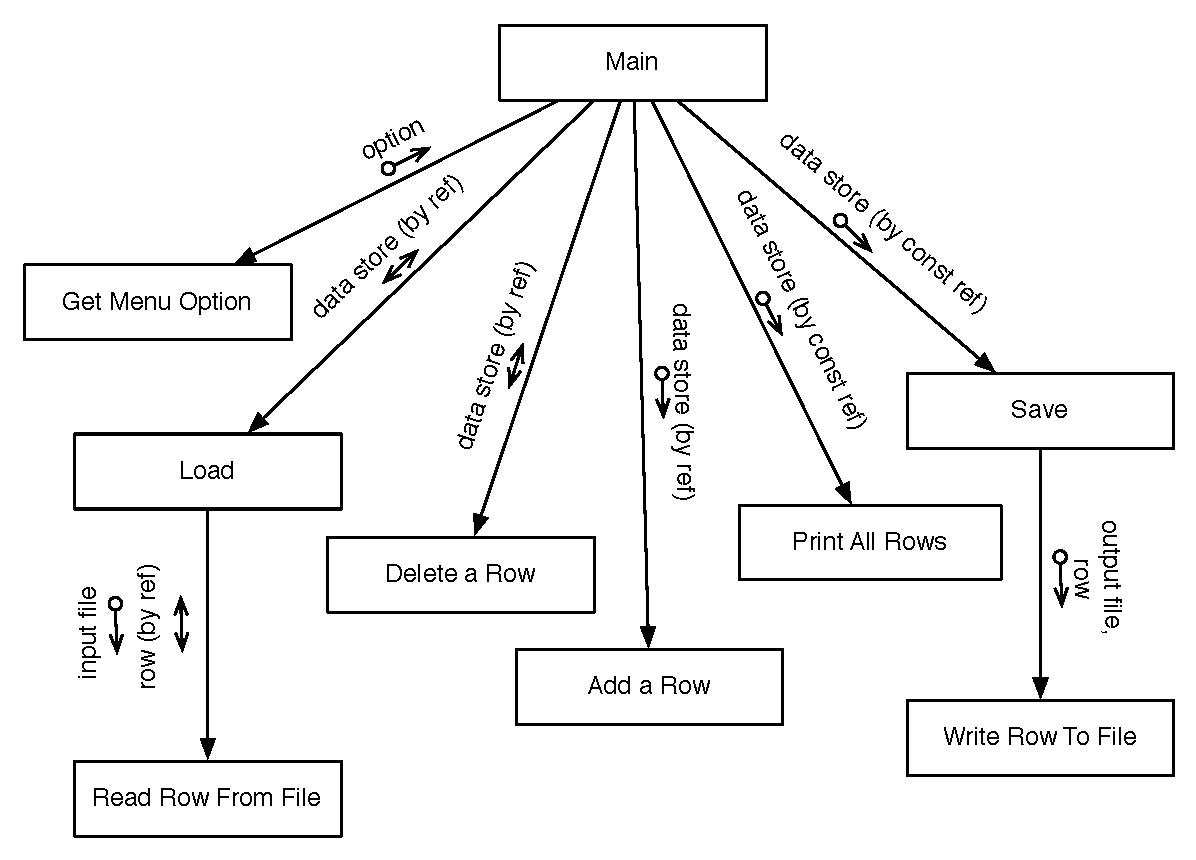
\includegraphics[width=\textwidth]{./topics/file-io/diagrams/SmallDB3Structure} 
   \caption{The structure chart showing the functions and procedures in Small DB}
   \label{fig:small_db_3_struct}
\end{figure}


% subsection new_structure_for_small_db (end)

\subsection{Writing Code to Load and Save Data for Small DB} % (fold)
\label{sub:writing_code_to_load_and_save_data_for_small_db}

Having completed the design for this version of the Small DB program, the next step is to covert these ideas into code. The pseudocode shown in this section communicate the logic that needs to be coded into the functions and procedures of the new version of the Small DB program. The following two sections, \sref{sec:file_io_in_c} \nameref{sec:file_io_in_c} and  \sref{sec:file_io_in_pascal} \nameref{sec:file_io_in_pascal}, contain a description of the tools needed to load and save data in the C and Pascal programming languages.

The good approach for implementing these additions will be to write the code to save the data to file first. Once you have this working you can run the program and check the file to see that the data you added was successfully saved. When this is working correctly you can move on to the code needed to read the values back from file. 

\fref{fig:small_db_3_running} shows the program running. Notice that that data remains the same even after quitting and running the program again. 


\begin{figure}[p]
   \centering
   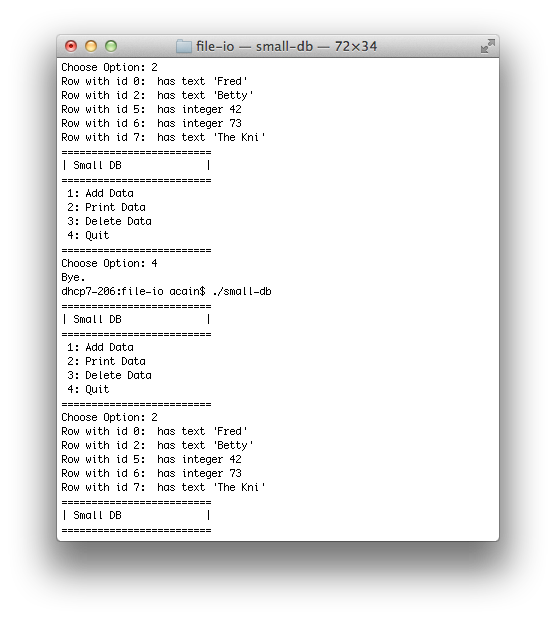
\includegraphics[width=0.9\textwidth]{./topics/file-io/images/SmallDBRunning} 
   \caption{Running Small DB program twice, notice the data persists between executions}
   \label{fig:small_db_3_running}
\end{figure}

\begin{figure}[p]
   \centering
   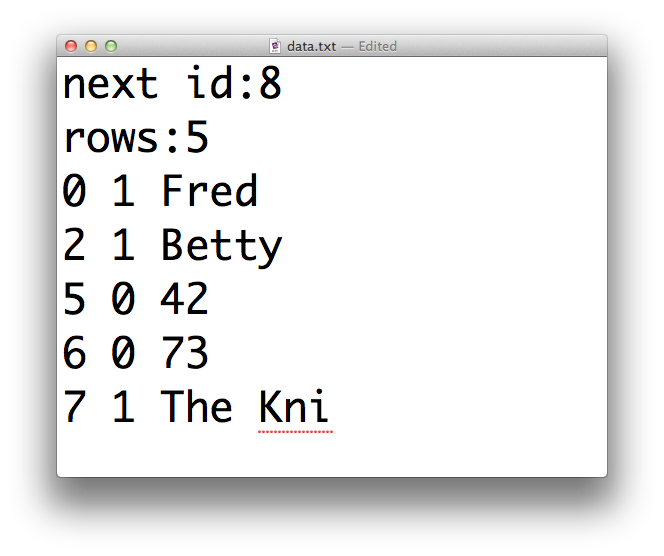
\includegraphics[width=0.3\textwidth]{./topics/file-io/images/DataText} 
   \caption{The contents of Small DB's data file, from \fref{fig:small_db_3_running}}
   \label{fig:small_db_3_data_text}
\end{figure}



% subsection writing_code_to_load_and_save_data_for_small_db (end)

% section using_input_and_output (end)
